\documentclass[pdf]{beamer}
\mode<presentation> {
   \usetheme{Warsaw}
}

\usepackage[slovak]{babel}
\usepackage[utf8]{inputenc}
\usepackage[IL2]{fontenc}
\usepackage{beamerprosper}
\usepackage{graphicx}
\usepackage{colortbl}
\usepackage{wrapfig}
\usepackage{subfig}
\usepackage{tikz}

\providecommand{\uv}[1]{\quotedblbase #1\textquotedblleft}
\providecommand\bi{\begin{itemize}}
\providecommand\ei{\end{itemize}}
\providecommand\li{\item}

\addtobeamertemplate{footline}{
  \setbeamertemplate{footline}[page number]
  \setbeamercolor{page number in head/foot}{use=headline,fg=headline.fg,bg=headline.bg}
  \usebeamertemplate{footline}
}{}

\definecolor{mylightblue}{rgb}{0.5,0.5,0.90}
\definecolor{highlight}{rgb}{1,1,0.5}


\begin{document}
	\usenavigationsymbolstemplate{}
	\title {Automatická kalibrácia kamery a lidaru}
	\subtitle{Projekt predmetu PGD}
	\institute{FIT VUT v~Brně\\\smallskip\texttt{\scriptsize ivelas00@fit.vutbr.cz}}
	\author {Martin Veľas}

	\begin{frame}
		\titlepage
	\end{frame}
	
	\begin{frame}{Motivácia}
		\begin{itemize}
			\item spojenie mračna bodov z lidaru (laserový radar, presná priestorová informácia) 
			\item a RGB kamery (farba)
		\end{itemize}
		\begin{block}{Využitie kalibrácie:}
			\begin{itemize}
				\item ofarbenie mračna bodov
				\item priradenie obrazových príznakov bodom mračna (lokalizácia, detekcia zmien, \ldots)
			\end{itemize}
		\end{block}
	\end{frame}
	
	\begin{frame}{Použité senzory}
		\begin{itemize}
			\item RGB kamera
			\item lidar \emph{Velodyne}
			\begin{itemize}
				\item horizontálny uhol $360^{\circ}$, vertikálny od $-10^{\circ}$ do $+30^{\circ}$
				\item hlava sa otáča s frekvenciou $10$Hz 				
				\item $32$ (resp. $64$ lúčov) a teda aj zosnímaných prstencov
				\item $700\,000$ zosnímaných bodov za sekundu
			\end{itemize}
		\end{itemize}	
		\begin{figure}[h]
			\center
			\subfloat{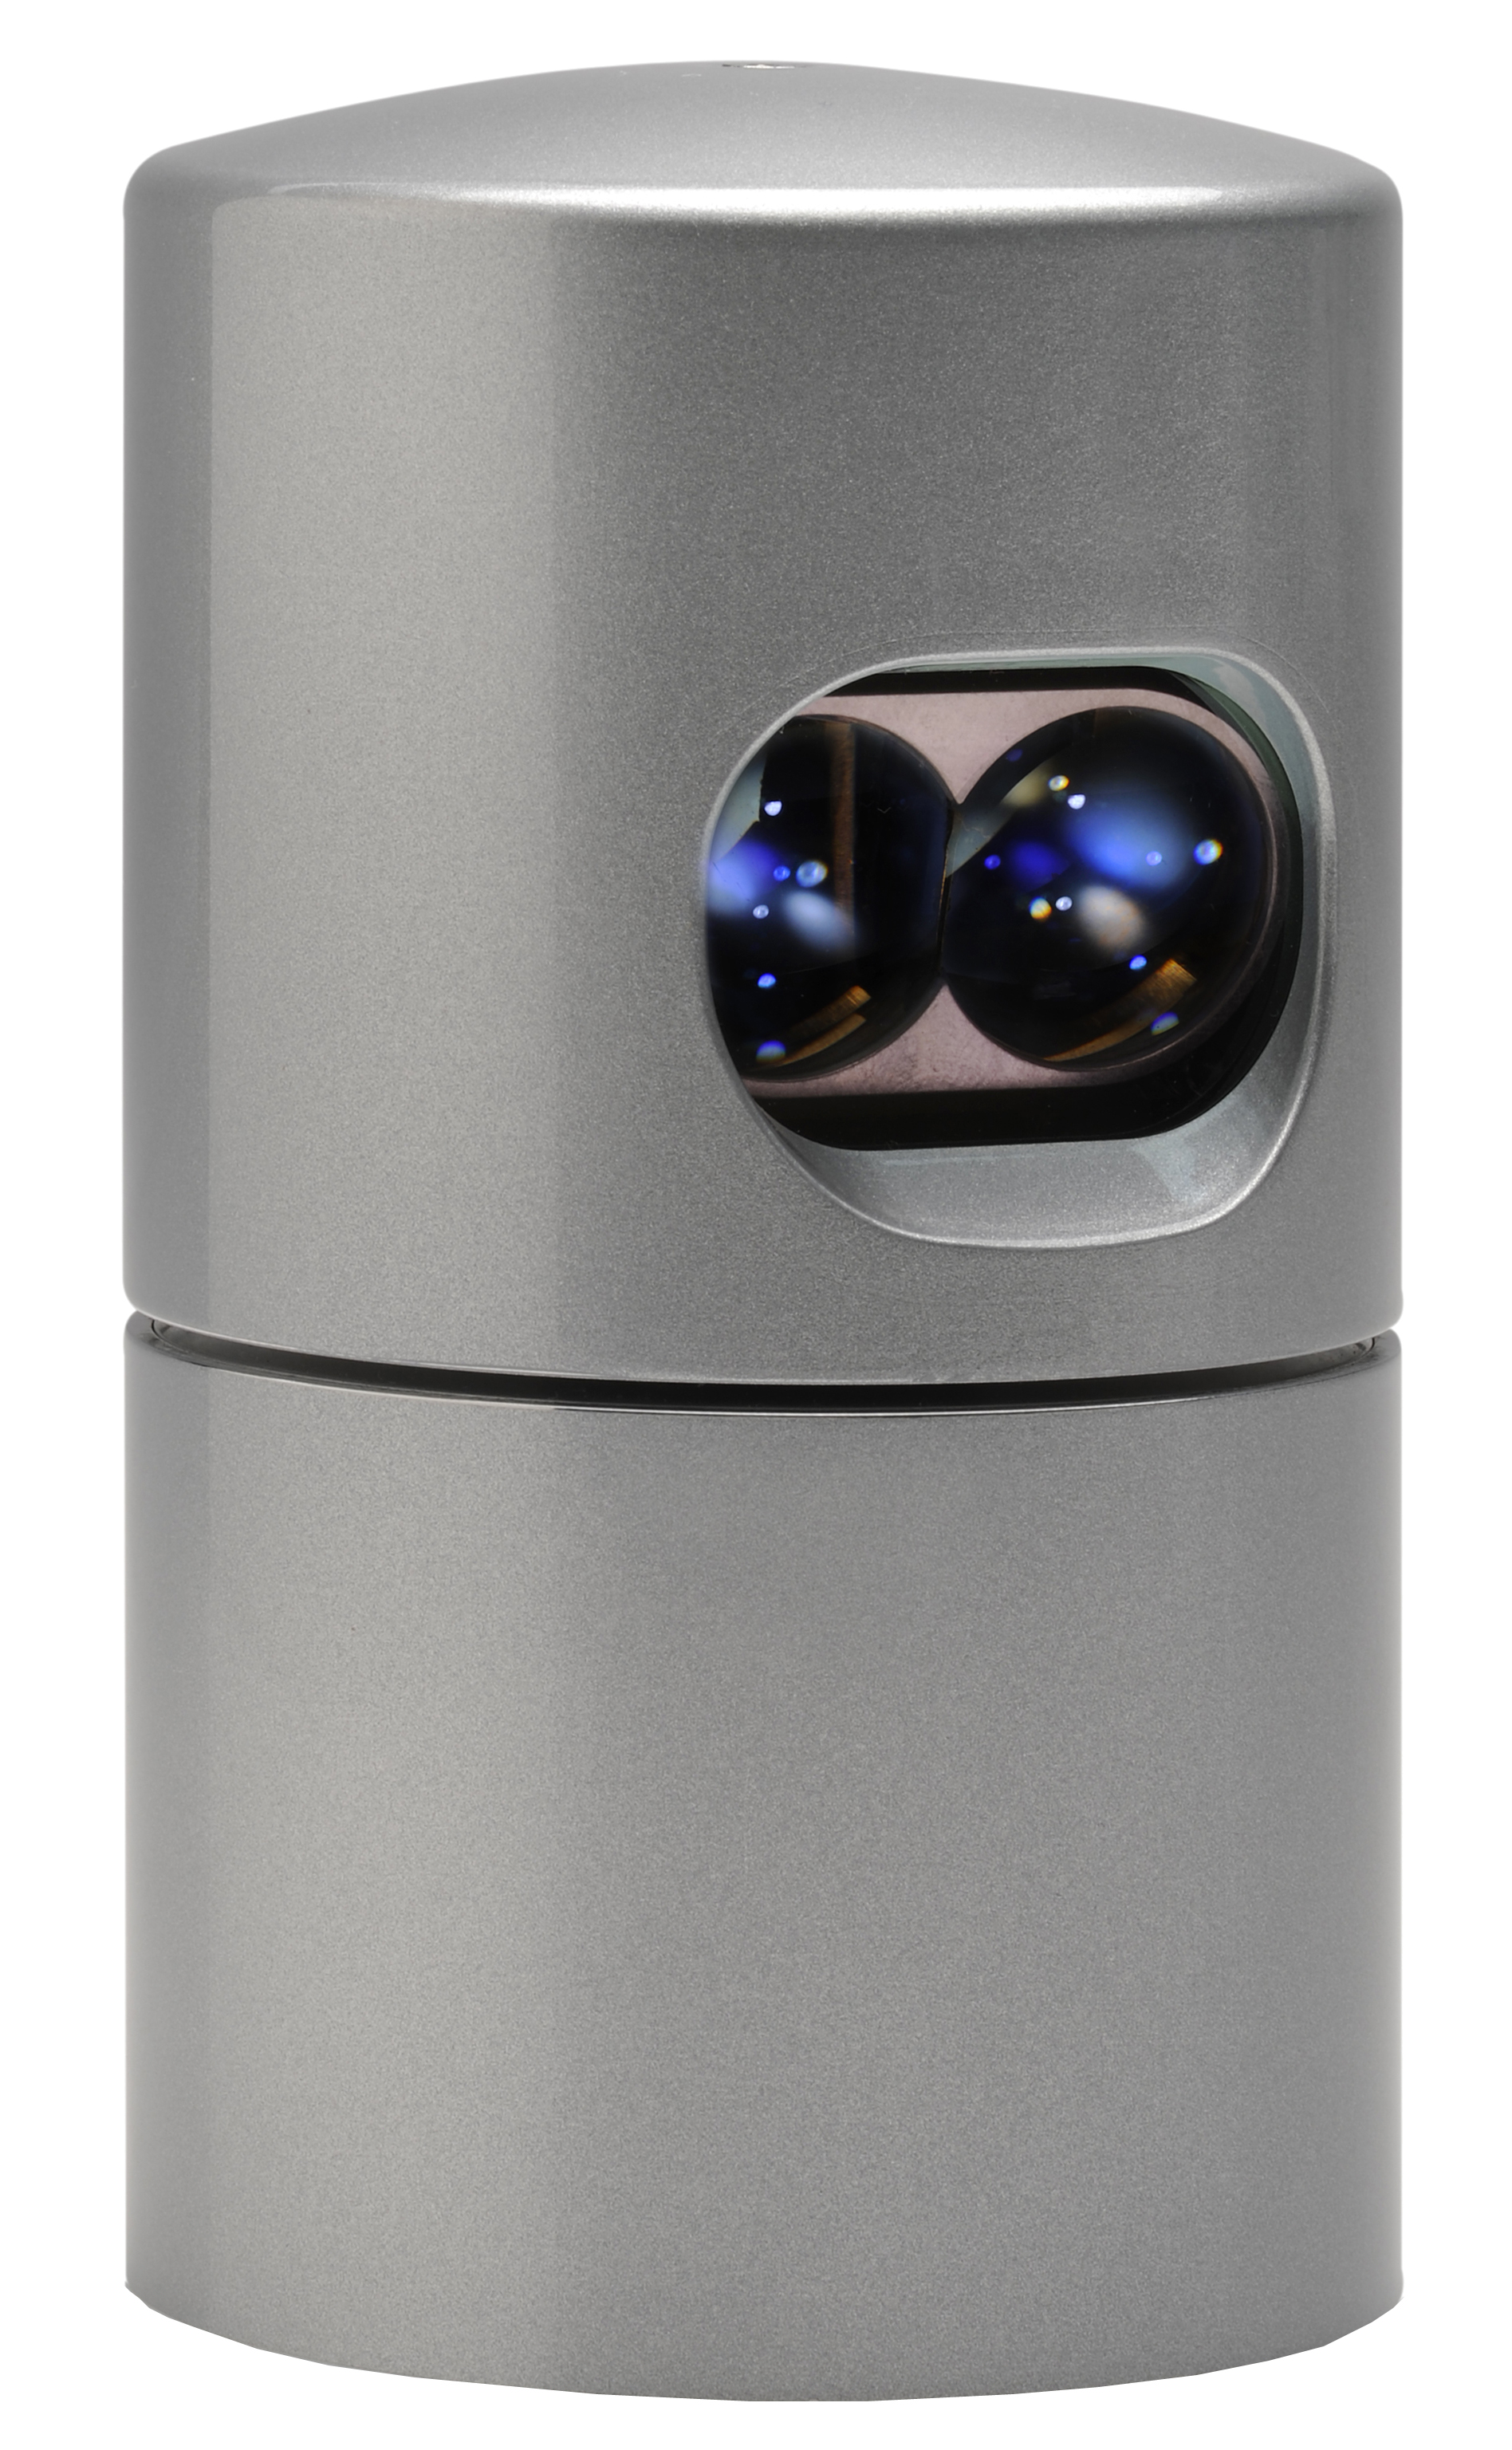
\includegraphics[height=0.25\textwidth]{../fig/velodyne_32.png}}
			\quad\quad\quad
			\subfloat{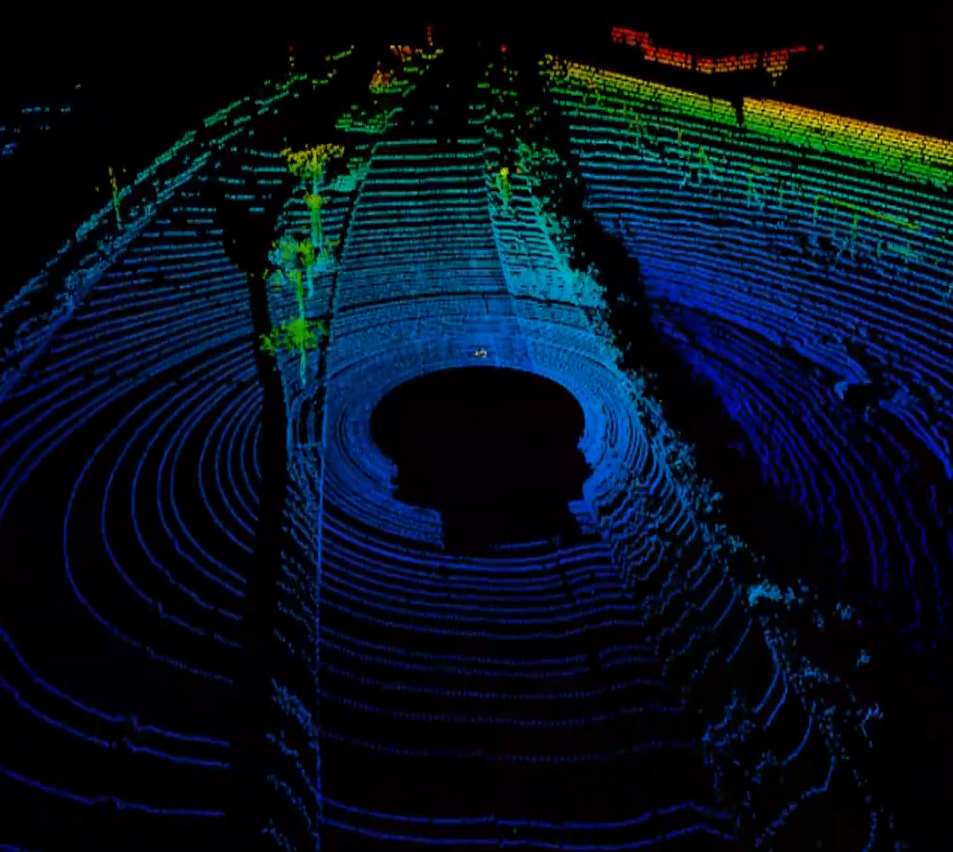
\includegraphics[height=0.25\textwidth]{../fig/velodyne_scan.png}}
		\end{figure}
	\end{frame}

	\begin{frame}{Velodyne}
		\begin{itemize}
			\item Video ukážka Velodyne \\
				\texttt{http://www.youtube.com/watch?v=P99eKc2uNJU}
		\end{itemize}
	\end{frame}
	
	\begin{frame}{Registrácia snímkov}
		\begin{itemize}
			\item určenie transformácie pre zarovnanie snímkov 
			\item Priama registrácia 
			\begin{itemize}
				\item detekcia bodov, extrakcia príznakov, matching, výpočet transformácie
				\item chýbajú príznaky $\Rightarrow$ nerealizovateľné
			\end{itemize}
			
			\item Registrácia ako optimalizácia
			\begin{itemize}
				\item potreba stanoviť kritérium -- hodnotiacu funkciu
				\item výber vhodnej optimalizačnej metódy (kvalita vs. výkon)
			\end{itemize}
		\end{itemize}
	\end{frame}
	
	\begin{frame}{Framework}
		\begin{figure}[h]
			\center
			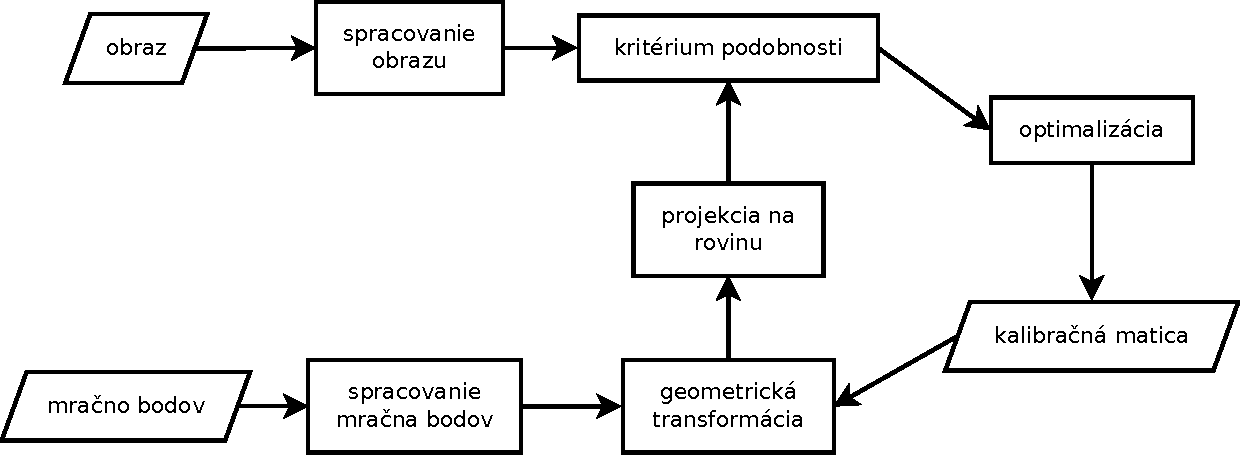
\includegraphics[width=0.99\textwidth]{framework.pdf}
		\end{figure}
	\end{frame}
	
	\begin{frame}{Geometrická transformácia}
		\begin{itemize}
			\item cieľom výpočtu je \emph{kalibračná matica}, ktorá transformuje body mračna do súradnicovej sústavy kamery
		\end{itemize}

		\begin{block}{Stupne voľnosti}
			\begin{itemize}
				\item $6$ \emph{Degrees of Freedom}
				\item posun v smere $x$, $y$ a $z$ osi
				\item rotácia okolo uvedených osí (roll, pitch, yaw)
			\end{itemize}
		\end{block}

		\begin{itemize}
			\item projekcia bodov mračna na rovinu 
			\item projekčná matica získaná podľa parametrov kamery
		\end{itemize}
	\end{frame}
	
	\begin{frame}{Registrácia založená na normálach}
		\begin{alertblock}{Predpoklad}
			\begin{itemize}
				\item plochy natočené smerom k zdroju svetla (typicky horizontálne) sú svetlejšie ako plochy odklonené
			\end{itemize}			
		\end{alertblock}		
		\begin{itemize}
			\item horizontálne plochy v mračne bodov teda odpovedajú oblastiam v obraze s vyššou intenzitou
			\item spracovanie obrazu -- prevod na odtiene šedej
		\end{itemize}
	\end{frame}
	
	\begin{frame}{Spracovanie mračna bodov}
		\begin{itemize}
			\item určenie normály v každom bode $c$ podľa bodov $p_i$ $8$ okolia
			\item výpočet kovariančnej matice:
				\begin{equation}
					C = \frac{1}{8} \sum\limits_{i=1}^8 (p_i-c)(p_i-c)^T
				\end{equation}.
			\item vlastný vektor s maximálnou vlastnou hodnotou zodpovedá normálovému vektoru
			\item uhol normály s horizontálnou plochou $x - z$ udáva intenzitu priradenú bodu
			\item možná ekvalizácia histogramu intenzít
		\end{itemize}
	\end{frame}

	\begin{frame}{Registrácia založená na normálach -- video}
		\begin{itemize}
			\item Video ukážka fúzie mračna bodov a RGB obrazu \\
				\texttt{http://www.youtube.com/watch?v=war\_cl0LdpI}
		\end{itemize}
	\end{frame}

	\begin{frame}{Registrácia založená na detekcii hrán}
		\begin{alertblock}{Predpoklad}
			\begin{itemize}
				\item hrany detekované v obraze sa prejavujú ako diskontinuity hĺbkového merania lidaru
			\end{itemize}			
		\end{alertblock}	
		\begin{itemize}
			\item v obraze a mračne bodov sú detekované hrany
			\item po priemete mračna na rovinu by hrany mali splynúť
		\end{itemize}			
	\end{frame}
	
	\begin{frame}{Detekcia hrán v obraze}
		\begin{itemize}
			\item vytvorenie hranového obrazu $E$
			\begin{itemize}
				\item hodnota pixelu je nahradená maximálnym rozdielom jeho intenzity a intenzity bodov v $8$ okolí
			\end{itemize}
			\item aplikácia \emph{Inversed Distance Transform (IDT)} pre vyhladenie výslednej hodnotiacej funkcie
			$$
				D_{i,j} = \alpha . E_{i,j} + (1-\alpha)\,.\,\underset{x,y}{max}\{ E_{x,y} . \gamma^{max(\vert x-i \vert, \vert y-j \vert)}\}
			$$
			\begin{figure}[h]
				\center
				\includegraphics[width=0.6\textwidth]{../fig/edges_idt.jpg}
			\end{figure}
		\end{itemize}
	\end{frame}

	\begin{frame}{Detekcia hrán v mračne bodov}
		\begin{itemize}
			\item hrany sa v snímku lidaru Velodyne prejavujú ako diskontinuity na prstencoch
			\item body mračna sú prechádzané po prstencoch a každému je priradená hodnota
				$$ X_i = max(P_{i-1}.r - P_i.r, P_{i+1}.r - P_i.r, 0)^\gamma $$
			\item prahovanie pre odstránenie šumu
		\end{itemize}
	\end{frame}
	
	\begin{frame}{Kritériá podobnosti}
		\begin{itemize}
			\item obraz a mračno bodov je spracovaný pomocou uvedených metód
			\item aplikácia geometrickej transformácie (kalibračná matica)			
			\item projekcia mračna na rovinu
			\item na výsledné obrazy je aplikované jedno z kritérií podobnosti
			\item hodnotiaca funkcia optimalizačnej úlohy
		\end{itemize}
	\end{frame}

	\begin{frame}{Kros-korelácia}
		\begin{itemize}
			\item jednoduché kritérium 
			\item pri porovnávaní obrazov rôznych modalít môže zlyhávať 
			\item skalárny súčin
			$$ C_{cc} = \sum\limits_i^W \sum\limits_j^H A_{i,j} . B_{i,j} $$
		\end{itemize}
	\end{frame}
	
	\begin{frame}{Mutual information}
		\begin{itemize}
			\item obraz je braný ako realizácia náhodnej veličiny
			\item ak je entropia obrazu definovaná ako 
			$$ H(X) = - \sum\limits_{i=1}^n p_i log(p_i) $$
			\item a spojená entropia obrazov 
			$$ H(X,Y) = - \sum\limits_{i=1}^n \sum\limits_{j=1}^m p_{i,j} log(p_{i,j}) $$
			\item potom normalizovanú vzájomnú informáciu definujeme ako
			$$ NMI(X,Y) = \dfrac{H(X) + H(Y)}{H(X,Y)} $$
		\end{itemize}
	\end{frame}
	
	\begin{frame}{Kalibrácia ako optimalizácia}
		\begin{itemize}
			\item uvedené kritéria podobnosti sa vyznačujú výraznými lokálnymi optimami
				\begin{figure}[h]
					\center
					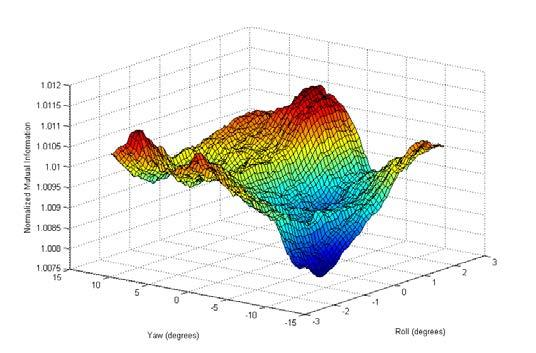
\includegraphics[width=0.5\textwidth]{../fig/nmi_values.jpg}
				\end{figure}
			\item metódy znižovania/zvyšovania gradientu nepoužiteľné
			\item kompletné prehľadávanie priestoru výpočetne nezvládnuteľné
			\item vhodný kompromis -- optimalizácie s prvkom náhodnosti (simulované žíhanie, particle swarm, \ldots)
		\end{itemize}
	\end{frame}
	
	\begin{frame}{Particle Swarm optimalizácia}
		\begin{itemize}
			\item roj častíc -- každá má pozíciu $x_i$ a zrýchlenie $v_i$
			\item všetky častice sa pohybujú v každej iterácii podľa vektoru zrýchlenia
			\item zrýchlenie sa v každej iterácii mení podľa
			\begin{itemize}
				\item predchádzajúceho zrýchlenia (interný faktor $w$), 
				\item pohybu k lokálne najlepšej nájdenej pozícii (kognitívny faktor $\phi_p$),
				\item pohybu ku globálne najlepšej nájdenej pozícii (sociálny faktor $\phi_g$)
			\end{itemize}
			\item výpočet zrýchlenia častice je ovplyvnený váhovaním náhodne generovanými premennými $c_p$ a $c_g$
		\end{itemize}	
	\end{frame}

	\begin{frame}{Zdroje}
		\begin{enumerate}
  			\item Levinson, J.; Thrun, S.: Automatic Online Calibration of Cameras and Lasers
  			\item Taylor, Z.; Nieto, J.: Automatic Calibration of Lidar and Camera Images using Normalized Mutual Information
  			\begin{figure}[h]
				\includegraphics[width=0.5\textwidth]{../fig/color_cloud.jpg}
			\end{figure}
  			\item Jan, J.: Medical Image Processing, Reconstruction and Restoration
  			\item Velodyne, http://velodynelidar.com/
  		\end{enumerate}
	\end{frame}
	
\end{document}
